\begin{figure}
    \centering
    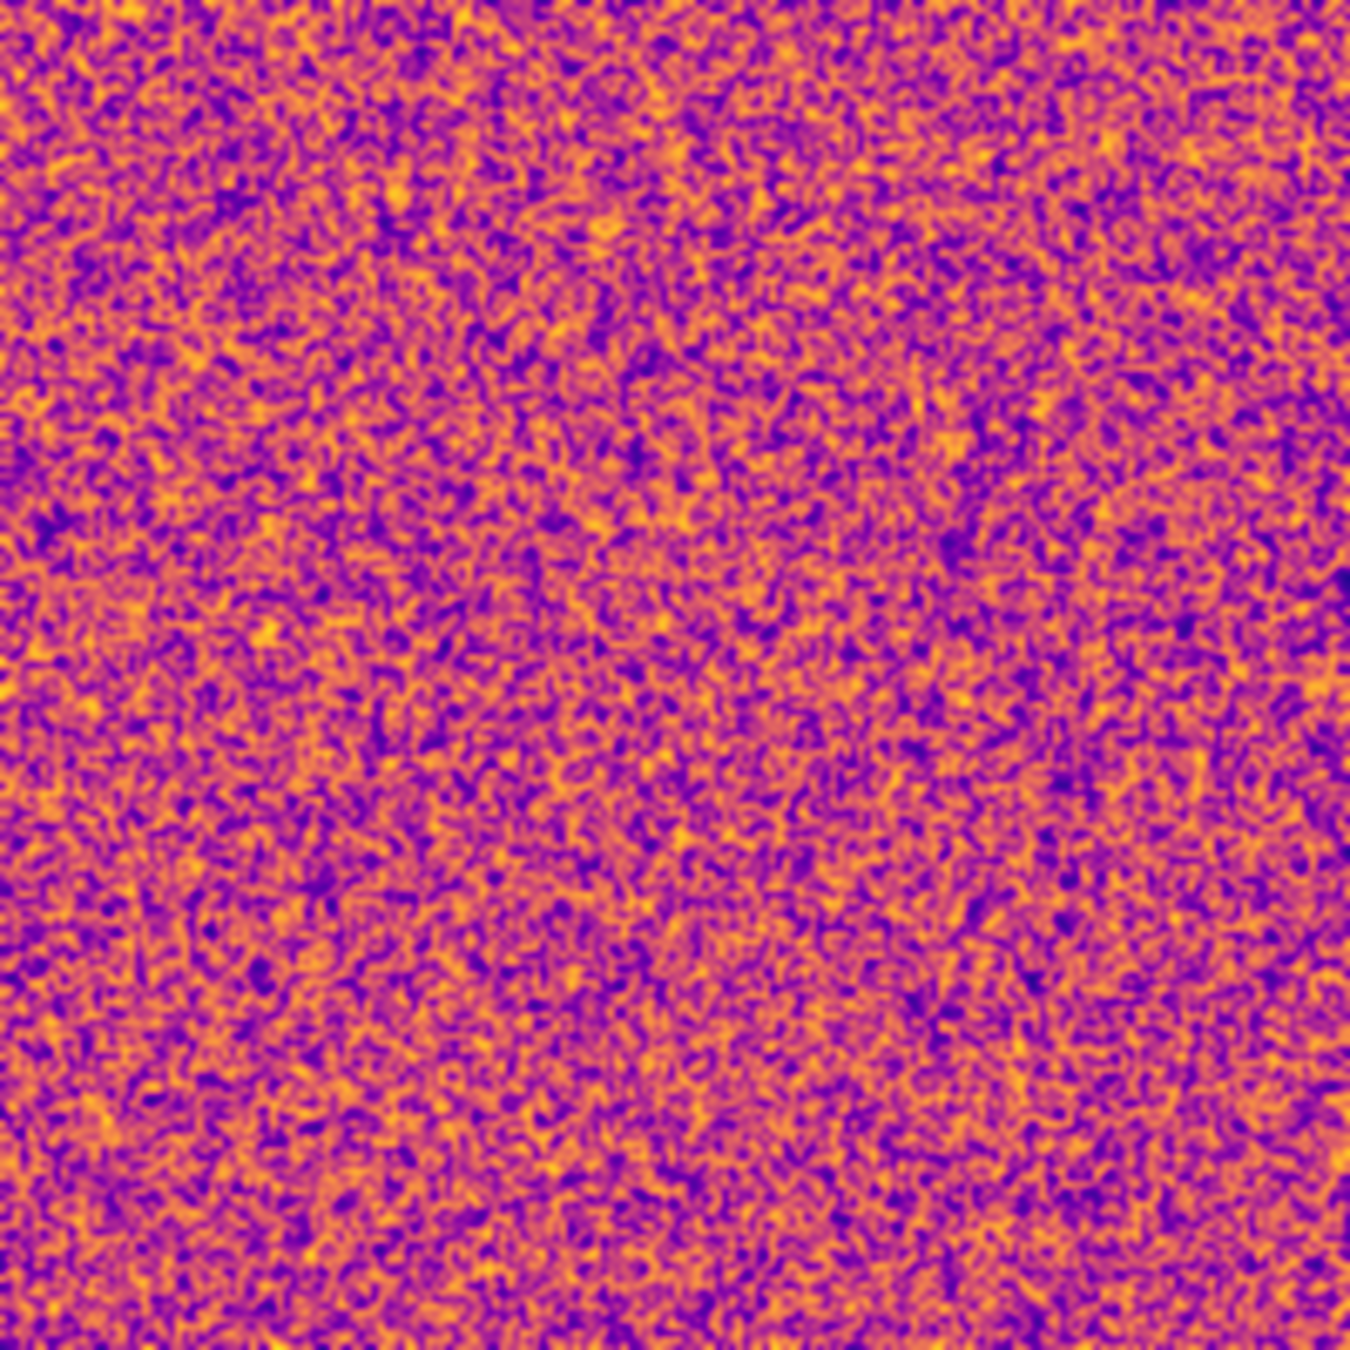
\includegraphics[width=0.32\linewidth]{papers/reaktdiff/images/LotkaVolterra/lv_n1.png}
    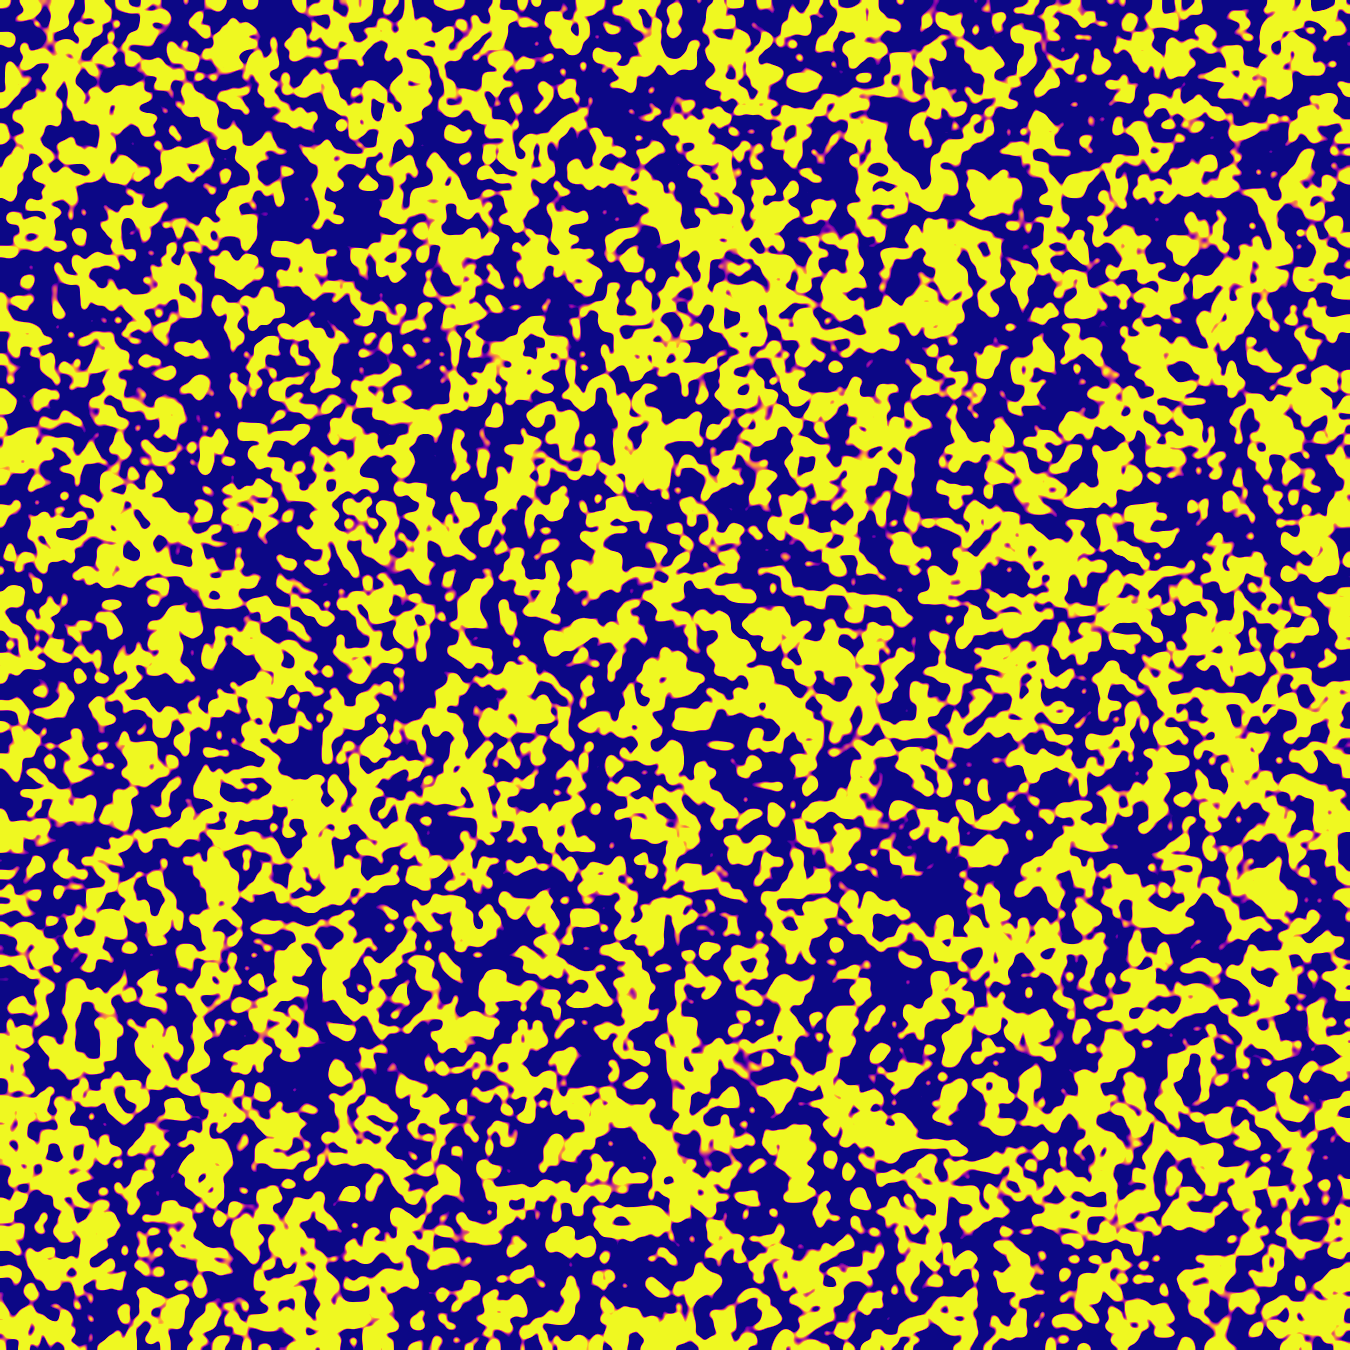
\includegraphics[width=0.32\linewidth]{papers/reaktdiff/images/LotkaVolterra/lv_n300.png}
    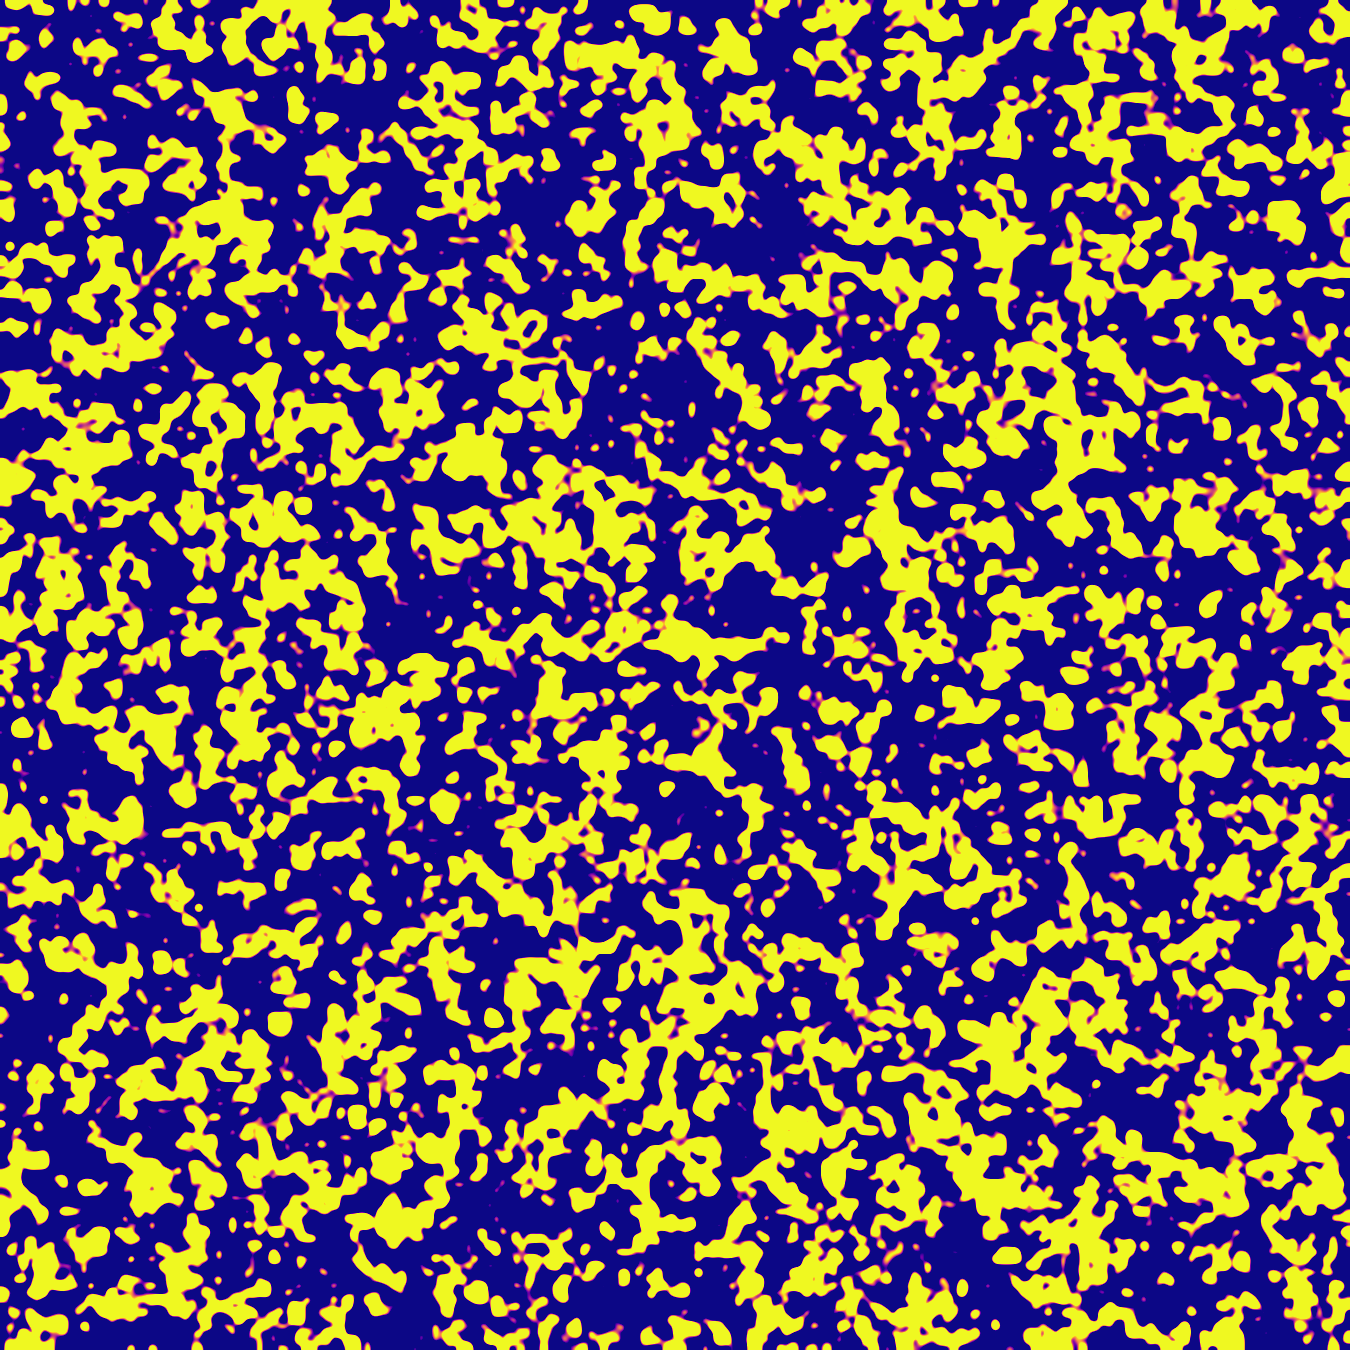
\includegraphics[width=0.32\linewidth]{papers/reaktdiff/images/LotkaVolterra/lv_n999.png}
    \caption{Verlauf der Simulation (von links nach rechts) der Reaktions-Diffusiongleichung mit Lotka-Volterra Modell \eqref{reaktdiff:equation:lvsys}
     als Reaktionsterm. Die erste Grafik zeigt den Anfangszustand. Die Oszillation ist in den Grafiken 2 und 3 angedeutet, jedoch schwer mit statischen Bilder darzustellen.}
    \label{reaktdiff:fig:lv}
\end{figure}
